This thesis explores the science and capabilities of ground based lightning detection networks.
What are lightning networks measurement limit?
How these networks are expanded and what are the results of these expansions?
Can choosing the right algorithm reveal larger structures from individual lightning locations?

With these questions lightning, thunderstorms, and the Earth-Ionosphere system are explored.
The electrical energy of thunderstorms is investigated in factors of production, how it discharges, where the energy goes, and how it contributes to the Earth system as a whole.

\section{Background}

\subsection{Lightning and Thunderstorms}

Lightning is the discharging of disparate charged regions in a thunderstorm.
When electrical charge is separated in a thunderstorm it can discharge, through lightning flashes, in order to neutralize the charge imbalance.

As deep convection develops in a thunderstorm, moist air is lifted from below the thunderstorm through the cloud where it condenses to above the freezing level.
Figure~\ref{intro:fig:thunderstorm} shows the basic components of an active thunderstorm.
The water begins to freeze as it passes through the freezing level of the thunderstorm; collisions at this freezing level occur with downwelling ice particles.
These collisions cause charge exchange between the downwelling ice, the ice gains a negative charge, and the upwelling graupel becomes positively charged.
This leads to the gross charge structure shown in Figure~\ref{intro:fig:thunderstorm}, with net positive charge in the top portion of the thunderstorm and net negative charge in the bottom portion.
There are smaller charge layers in the thunderstorm, such as screening layers, but the overall charge structure is that depicted in Figure~\ref{intro:fig:thunderstorm}.

\begin{figure}[ht!]
	\centering
	\includegraphics[scale=1]{Introduction/Figures/thunderstorm_structure.pdf}\\
	\caption{Overall thunderstorm charge structure, showing a typical freezing level and tropopause hight.}
	\label{intro:fig:thunderstorm}
\end{figure}

The lightning discharge begins with the stepped-leader process.
While a voltage on the order of 1~MV builds up between the charge centers (e.g. the thunderstorm and ground) it is still far less than the breakdown electric field of air (on the order of 1~MV/m).
However the air can be broken down in $\sim$100~m steps, creating a continuous ionized plasma channel; the breakdown process is semi-random with steps occurring until an oppositely charge region is connected.
An example of a step-leader breakdown is shown at the beginning of Figure~\ref{intro:fig:evolution}.

For the first $\sim$20~ms the step leader creates the ionized channel to ground (or to another charge region).
Once the channel is established the return stroke moves charge from the ground to the cloud over the course of $\sim$70~$\mu$s (the return stroke labelled in Figure~\ref{intro:fig:evolution}).
After the return stroke occurs the top of the ionized channel can connect to other charge regions through a subsequent step-leader process, producing multiple return strokes along the same ionized channel.
The total process, from step-leader through multiple return strokes, is considered a single lightning flash.

\begin{figure}[ht!]
	\centering
	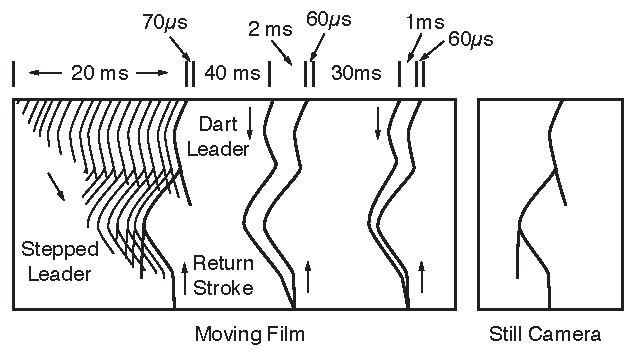
\includegraphics[scale=1]{Introduction/Figures/Lightning_Evolution.pdf}\\
	\caption{The step-leader and discharge process of cloud to ground lightning with typical times of each event (adapted from \citet{Uman1969}). Timing not to scale.}
	\label{intro:fig:evolution}
\end{figure}

Lightning can discharge in several configurations, the most common shown in Figure~\ref{intro:fig:types}.
Lightning predominately occurs either between clouds or within the same cloud, called: cloud-to-cloud lightning, in-cloud lightning, or cloud lightning (Figure~\ref{intro:fig:types}c and~\ref{intro:fig:types}f).
Lightning between the thunderstorm and ground is more powerful, easier to detect, and less common.
It can occur in 4 combinations of positive or negative charge in the cloud discharging to ground with the discharge beginning in the cloud or on the ground (Figure~\ref{intro:fig:types}a, \ref{intro:fig:types}b, \ref{intro:fig:types}d, and~\ref{intro:fig:types}d).
Negative cloud to ground lightning (moving negative charge from the cloud to ground, Figure~\ref{intro:fig:types}a) is the most common cloud-to-ground discharge at a ratio of 10:1.
It is estimated that there are 4 in-cloud (IC) strokes (or flashes) for every cloud-to-ground (CG) stroke \citep{Uman1969}.

\begin{figure}[ht!]
	\centering
	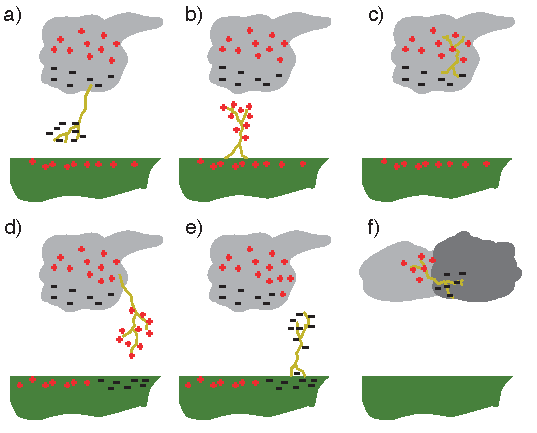
\includegraphics[scale=1]{Introduction/Figures/lightning_types.pdf}\\
	\caption{Different types of lightning discharges:
			a) negative cloud-to-ground,
			b) positive ground-to-cloud,
			c) in-cloud,
			d) positive cloud-to-ground,
			e) negative ground-to-cloud,
			f) cloud-cloud.
			Note that a) and b) produce the same overall charge movement (negative charge to ground) and conversely for d) and e).
			 (Based on \citet{Uman1969})}
	\label{intro:fig:types}
\end{figure}

There are other sources for large electrical discharges similar to thunderstorm lightning.
For example there are electrical discharges that produce electromagnetic waves similar to lightning: terrestrial gamma ray flashes, terrestrial luminous events, volcanic lightning, and compact intra-cloud discharges.
However these events are less common than typical lightning and will not be considered here.

\subsection{The Ionosphere}

The ionosphere is the plasma environment located between 80~km and 1000~km altitude, it is a highly conductive region within the exponentially decreasing atmospheric neutral density.
It forms from the ionization of the background neutral particles by ultraviolet sunlight.
During the day the ionospheric D- and E-regions extend farther down in altitude than during night when the ions recombine and disappear, shown in Figure~\ref{intro:fig:ionosphere}.
High altitudes in the F-region remain through the night as the particle density is much lower, preventing significant recombination.

\begin{figure}[ht!]
	\centering
	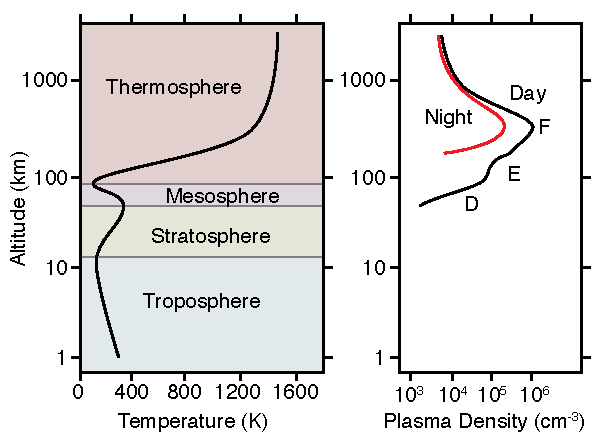
\includegraphics[scale=1]{Introduction/Figures/ionosphere.pdf}\\
	\caption{Atmospheric temperature profile and ionospheric plasma density profile (day ionosphere in black, night ionosphere in red).
		     }
	\label{intro:fig:ionosphere}
\end{figure}

At very low frequency waves (1~kHz to 24~kHz) the conductive ionosphere and ground are good reflectors and form the Earth-Ionosphere Wavegude (EIWG).
The EIWG allows for propagation of VLF waves from natural sources (e.g. lightning) and artificial sources (e.g. Navy VLF transmitters) to propagate large distances ($>5000$~km).
VLF waves propagating in the waveguide undergo loss on the order of 1~dB/Mm, with the lost energy  heating the waveguide (mostly the ionosphere) and generating plasma waves in the ionosphere (Figure~\ref{intro:fig:eiwg}).
VLF wave attenuation is greatest over ice, then continents, with the lowest attenuation over the oceans.

\begin{figure}[ht!]
	\centering
	\includegraphics[scale=1]{Introduction/Figures/eiwg.pdf}\\
	\caption{Schematic of the Earth-Ionosphere Waveguide.}
	\label{intro:fig:eiwg}
\end{figure}

\subsection{Global Electric Circuit}

The global electric circuit is the current system formed by the ionosphere and ground acting as a leaky spherical capacitor, as shown in Figure~\ref{intro:fig:gec}a, with an equivalent circuit shown in Figure~\ref{intro:fig:gec}b.
Thunderstorms are the primary drivers of the global electric circuit with the charged ionosphere discharging through fair weather atmosphere.
The global circuit was first proposed after observing diurnal variation in global thunderstorm activity along with fair weather electric field measurements, originally observed by \citet{Wilson1921} and \citet{Whipple1929}.
Strong correlations between thunderstorm activity and fair weather return current led to the current model of the global electric circuit.
The global electric circuit activity changes on short time scales that are not resolved with past models or with long term averaged observations \citep{Holzworth1984a}.
The global electric circuit is an important component to the solar-terrestrial system creating a link between solar activity, the ionosphere, aerosols, cloud microphysics, thunderstorms, weather, and climate \citep{Tinsley2007, Holzworth1986}.

\begin{figure}[ht!]
	\centering
	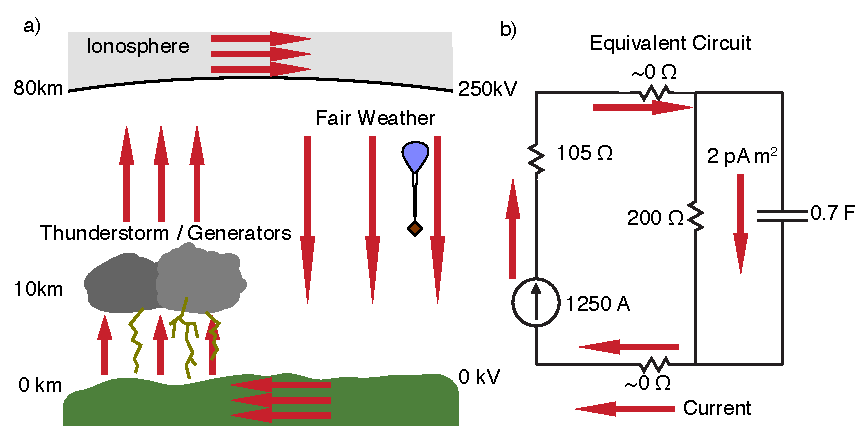
\includegraphics[scale=1]{Introduction/Figures/global_circuit.pdf}\\
	\caption{a) Global electric circuit model, arrow correspond to currents.
			b) Circuit equivalent model with representative values.}
	\label{intro:fig:gec}
\end{figure}

\section{Lightning Detection Systems}

There is a growing importance, both scientifically and operationally, of ground based lightning detection networks.
Lightning detection networks are being used in a larger gamut of research areas including: terrestrial gamma ray flashes \citep{Dwyer2012, Gjesteland2011, Connaughton2010}, lightning climatology \citep{Virts2013, Virts2011a, Burgesser2012}, ionospheric disturbances and probing \citep{Jacobson2010, Singh2011}, transient luminous events \citep{Soula2011}, global electric circuit  \citep{Holzworth2005}, and whistler observation \citep{Collier2010, Collier2011a, Burkholder2013}.
This is in conjunction with the extended usage of lightning networks operationally in weather prediction and tracking \citep{Fierro2012, Pan2010, Thomas2010d}, volcano monitoring \citep{Doughton2010}, and hazard estimation \citep{Altaratz2010}.
With growing usage it is necessary to understand the capabilities and efficiencies of the various available lightning networks.

Ground based total lightning networks distinguish themselves from other ground based networks and satellites by detecting and identifying in-cloud (IC) discharges as well as cloud to ground (CG) strokes.
Lightning type is critical in understanding thunderstorm dynamics \citep{Williams1989}, with real time monitoring of sudden increases of IC activity able to predict severe weather events \citep{Rudlosky2013, Darden2010, Metzger2013, Schultz2009, Schultz2011}.
The higher frequencies of total lightning networks are also useful for researching narrow bipolar events \citep{Suszcynsky2003} and large scale lightning behavior \citep{Hutchins2013}.
Lightning mapping arrays are able to locally detect, locate, and distinguish IC activity, however total lightning networks have the advantage of much larger spatial coverage.

\subsection{World Wide Lightning Location Network}

The World Wide Lightning Location Network (WWLLN, see http://wwlln.net) determines the location for nearly all lightning producing storms around the globe in real time \citep{Jacobson2006c}.
WWLLN has been generating global lightning locations starting in 2004 \citep{Rodger2006, Rodger2009}, since then the network has grown from 18 stations to over 70 as of April 2014.
Knowledge of individual stroke locations, with high temporal accuracy and within a fraction of a wavelength, is beneficial for both scientific and technical uses.
WWLLN lightning location data have recently been used for advances in space science \citep{Lay2007, Kumar2009, Collier2009, Holzworth2011, Jacobson2011}, meteorology \citep{Price2009,Thomas2010d}, detailed lightning physics \citep{Connaughton2010}, and volcanic eruption monitoring \citep{Doughton2010}.
The observed global lightning stroke density for 2011 -- 2012 is shown in Figure~\ref{intro:fig:wwlln}.

\begin{figure}[ht!]
	\centering
	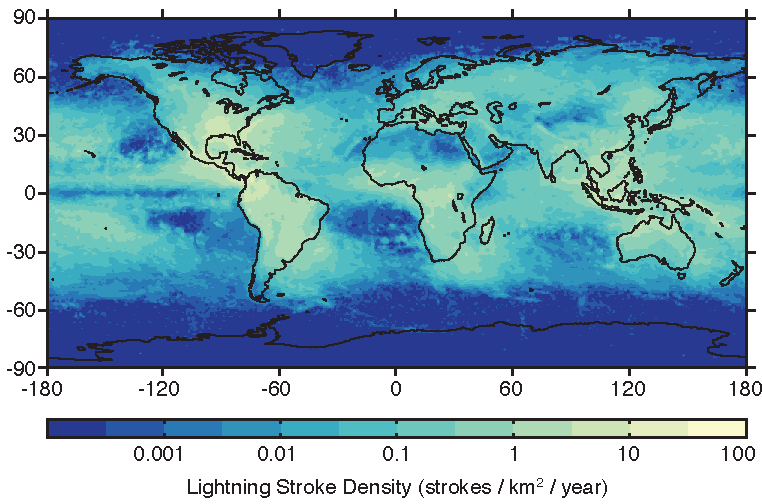
\includegraphics[scale=1]{Introduction/Figures/wwlln_density.pdf}\\
	\caption{Global WWLLN lightning stroke density for 2011 -- 2012.}
	\label{intro:fig:wwlln}
\end{figure}

The network uses a time of group arrival (TOGA) technique, originally developed by \citet{Dowden2002d}, to locate strokes by analyzing the sferic waveforms at each station using the Stroke\_B algorithm as discussed by \citet{Rodger2006,Rodger2009}.
WWLLN locates strokes by analyzing the TOGA of the sferic wave packet in the 6 -- 18~kHz band \citep{Dowden2000}.
The TOGA of the VLF wave packet, is used rather than the trigger time to produce more uniform arrival times across the network.
A recent upgrade to the network allows for the measurement of the radiated VLF energy of located strokes within the 8 -- 18~kHz VLF band (see Chapter~\ref{thesis:chapter:energy}).
The stroke energy is calculated from the square root of the time-integrated squared (RMS) electric field of the VLF sferic at each WWLLN station, using the Long Wave Propagation Capability code (\citet{Ferguson1998}, see \ref{intro:sec:lwpc}) to estimate the sferic attenuation and calculate the source radiated energy \citep{Hutchins2012}.

As stations are added the accuracy and detection efficiency of the network improves.
In 2010 the network locates most strokes to within 10~km and $<$10~$\mu$s with an estimated detection efficiency of about 11\% for all strokes and $>$30\% for more powerful strokes \citep{Abarca2010,Rodger2009}.
The network improves in accuracy and detection efficiency with increased stations; for example an increase in the number of WWLLN stations from 11 in 2003 to 30 in 2007 led to a $\sim$165\% increase in the number of lightning strokes located \citep{Rodger2009}.
However the WWLLN network does not observe lightning with the same detection efficiency everywhere.
This is due to variable WWLLN station coverage and the strong effect on VLF radio propagation from surface electrical conductivity and ionospheric conditions along the great-circle path of the wave.

\subsection{Earth Networks Total Lightning Network}

The Earth Networks Total Lightning Network (ENTLN) is a ground based network that began in 2009 as the Weatherbug Total Lightning Network (WTLN).
It has two operational regimes: short range using broadband sferic waveforms (5~kHz -- 12~MHz) and long range with only VLF/LF waveforms (1~Hz -- 256~kHz) \citep{Heckman2010}.
Correlations of the stroke waveform and amplitude from multiple stations determines the time, location, altitude, peak current, polarity, and type of the located stroke \citep{Liu2011a}.
The network utilizes a time of arrival method to determine the location of each stroke, where a minimum of 8 stations is required to produce a valid solution.
To compress the broadband waveforms each station removes the necessary amount of low-amplitude signal to reach the requisite packet size.
In the continental United States (CONUS) the network has approximately 530 operational stations in September 2013.
A comparison to the Oklahoma Lightning Mapping Array (OKLMA) in 2010 demonstrated the ability to discriminate between CG and IC strokes \citep{Beasley2010}.
The observed stroke density over North America for 2011 -- 2012 is shown in Figure~\ref{intro:fig:entln}.

\begin{figure}[ht!]
	\centering
	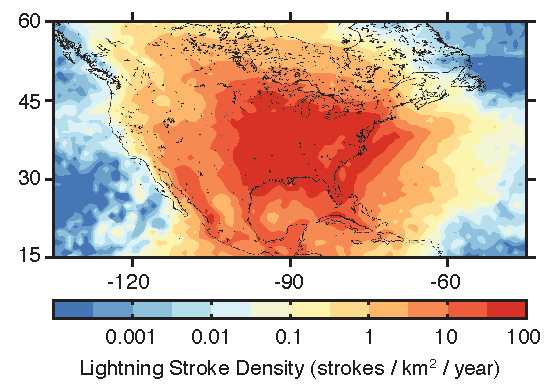
\includegraphics[scale=1]{Introduction/Figures/entln_density.pdf}\\
	\caption{North American ENTLN lightning stroke density for the 2011 -- 2012 dataset.
	              Note same range as Figure~\ref{intro:fig:wwlln}}
	\label{intro:fig:entln}
\end{figure}

\subsection{TRMM/LIS}

The Lightning Imaging Sensor (LIS, 1997-present) is a satellite-based lightning detector flown onboard the Tropical Rainfall Measurement Mission (TRMM) satellite orbiting at a 35$^\circ$ inclination and 402~km altitude \citep{Christian1999}.
In low earth orbit it observes the total lightning activity from individual thunderstorms for 90 sec in each $0.5^\circ \times 0.5^\circ$ viewtime granule.
LIS is useful as it is an optical lightning detection system without the spatial dependency inherent with ground based networks, and the sensor performance has not changed over time.
The LIS data are available at several processed levels, throughout this work the flash level data is used.
The LIS flash density for 2011 -- 2012 is shown in Figure~\ref{intro:fig:lis}.

\begin{figure}[ht!]
	\centering
	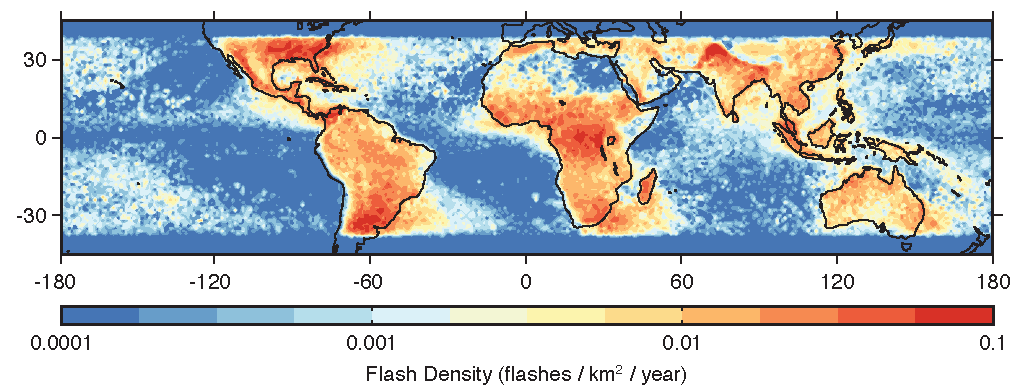
\includegraphics[scale=1]{Introduction/Figures/lis_density.pdf}\\
	\caption{LIS lightning flash density for 2011 -- 2012.
		     Note the reduced range from Figures~\ref{intro:fig:wwlln} and~\ref{intro:fig:entln}}
	\label{intro:fig:lis}
\end{figure}

\section{Long Wave Propagation Capability Code}
\label{intro:sec:lwpc}

The Long Wave Propagation Capability code (LWPC) is used to model the VLF attenuation between WWLLN located lightning and the network stations.
The LWPC code was developed by the Space and Naval Warfare Systems Center by \citet{Ferguson1998} and has most recently been validated by \citet{McRae2000d} and \citet{Thomson2011}.
In this research we made use of an adapted LWPC version 2.1 (available online, see Appendix~\ref{thesis:appendix:code}).

LWPC can be used to model the attenuation along a mixed day/night ionospheric path, however due to computational limitations a lookup table is used instead.
The lookup tables model the received electric field at a given station for a 100~kW transmitter in each grid cell.
A $1^{\circ}$ by $1^{\circ}$ grid is used for either an all day ($\beta=0.3$ km$^{-1}$ and $h'=74$ km) or an all night ($\beta(f)=0.3-0.8$ km$^{-1}$ and $h'=87$ km) ionospheric model, where $\beta$ and $h'$ are the slope of the conductivity ($\beta$ is frequency dependent at night) and the reference height.
The ionospheric models are the default models of LWPC and fully described in \citet{Ferguson1998}.

For each grid cell the electric field is averaged over the 8 -- 18 kHz band, which captures the frequencies of the peak radiated power from lightning \citep{Volland1995}.
An example of the day ionosphere lookup table for the Dunedin station is shown in Figure~\ref{intro:fig:lookup}.
The discontinuity of electric field over Greenland and in the South Atlantic is caused by the high attenuation rate of VLF propagating over ice.
Using the lookup tables assumes that the attenuation rates do not vary greatly within a given grid cell and that the frequency response of a sferic is relatively flat within the band considered.

\begin{figure}[ht!]
	\centering
	\includegraphics[scale=1]{Introduction/Figures/lwpc_Lookup.pdf}\\
	\caption{LWPC generated lookup table for Dunedin station (white triangle) using an all day ionospheric model ($	\beta=0.3$ km$^{-1}$ and $h'=74$ km) averaged over 8 -- 18~kHz. Each $1^{\circ}$ by $1^{\circ}$ bin shows the electric field seen at Dunedin if a 100kW transmitter is centered on that bin.}
	\label{intro:fig:lookup}
\end{figure}

\section{Outline}

An outline of this work is provided in Table~\ref{intro:table:outline}, along with the corresponding publications adapted by each chapter.
Chapters~\ref{thesis:chapter:energy} -- \ref{thesis:chapter:entln-lis} cover the technical improvements and analysis of the networks used, work that is necessary for the following chapters.

\begin{table}[ht!]
\caption{Chapter outline.}
\label{intro:table:outline}
\begin{center}
\begin{tabular}{l p{4in} l}

\rule{0pt}{3ex}
Chapter~\ref{thesis:chapter:energy}	&
Describes the process for calculating the far-field radiated VLF energy of lightning with WWLLN.	&
\citet{Hutchins2012}\\ 

% \hline
\rule{0pt}{3ex}
Chapter~\ref{thesis:chapter:efficiency}	&
Discusses the relative detection efficiency model of WWLLN.	&
\citet{Hutchins2012a}\\ 

% \hline
\rule{0pt}{3ex}
Chapter~\ref{thesis:chapter:entln-lis}	&
Examines the detection efficiency between the ENTLN and LIS lightning data over North America.	&
Under Review\\ 

% \hline
\rule{0pt}{3ex}
Chapter~\ref{thesis:chapter:landsea}	&
Examines the energy contrast between oceanic and continental lightning using a linear regression method developed in the chapter.	&
\citet{Hutchins2013}\\ 

% \hline
\rule{0pt}{3ex}
Chapter~\ref{thesis:chapter:prop} &
Combines the WWLLN energy measurements with network station electric field measurements to estimate the VLF attenuation rates over ocean under the day and night ionosphere.
& \citet{Hutchins2013a}.\\

% \hline
\rule{0pt}{3ex}
Chapter~\ref{thesis:chapter:gec} &
Applies a clustering algorithm to the WWLLN stroke locations, producing thunderstorm clusters, to create a prediction of the global electric circuit activity.
& \citet{Hutchins2014}.\\

% \hline
\rule{0pt}{3ex}
Chapter~\ref{thesis:chapter:thunderstorm}&
The thunderstorm clustering is expanded to flash clustering and explored in the context of matching efficiency. &
\\

% \hline
\rule{0pt}{3ex}
Chapter~\ref{thesis:chapter:conclusion} &
Explores the future work that can be carried forward from this work. &
\\

\end{tabular}
\end{center}
\end{table}

The appendices discuss the code implementation of the techniques described in a few of the chapters and the construction, design, and operation of the WWLLN stations.
Their descriptions are given in Table~\ref{intro:table:outline_appendix}.
Notably the code for the energy calculations (Chapter~\ref{thesis:chapter:energy}), relative detection efficiency model (Chapter~\ref{thesis:chapter:efficiency}), and thunderstorm clustering (Chapter~\ref{thesis:chapter:gec}) are available online as described in Appendix~\ref{thesis:appendix:code}.  The same appendix contains the schematics, EAGLE files, parts list, and software for the WWLLN Service Units.

\begin{table}[ht!]
\caption{Appendix outline.}
\label{intro:table:outline_appendix}
\begin{center}
\begin{tabular}{l p{5in}}

\rule{0pt}{3ex}
Appendix~\ref{thesis:appendix:code}	&
Describes the different types of WWLLN data files available, their location, and the common code used in this thesis (code for individual chapters can be made available upon request).
\\ 

\rule{0pt}{3ex}
Appendix~\ref{thesis:appendix:energy} &
Describes the WWLLN stroke energy processing code and operations, enabling reproduction or reprocessing of the energies.
\\ 

\rule{0pt}{3ex}
Appendix~\ref{thesis:appendix:su}	&
Describe the development, design, and construction of the WWLLN Service Unit v4.
\\  

\rule{0pt}{3ex}
Appendix~\ref{thesis:appendix:gumstix}	&
Describes the software and operations of the WWLLN Service Unit v4 computers.
\\ 

\rule{0pt}{3ex}
Appendix~\ref{thesis:appendix:website}	&
Outlines the new WWLLN website structure and operation along with the realtime lightning display.
\\ 

\end{tabular}
\end{center}
\end{table}
